\documentclass[11pt]{article}
\usepackage[utf8]{inputenc}	% Para caracteres en español
\usepackage{amsmath,amsthm,amsfonts,amssymb,amscd}
\usepackage{multirow,booktabs}
\usepackage[table]{xcolor}
\usepackage{fullpage}
\usepackage{lastpage}
\usepackage{enumitem}
\usepackage{fancyhdr}
\usepackage{mathrsfs}
\usepackage{wrapfig}
\usepackage{setspace}
\usepackage{calc}
\usepackage{multicol}
\usepackage{cancel}
\usepackage{float}
\usepackage{physics}
\usepackage[retainorgcmds]{IEEEtrantools}
\usepackage[margin=1cm]{geometry}
\usepackage{amsmath}
\newlength{\tabcont}
\setlength{\parindent}{0.0in}
\setlength{\parskip}{0.05in}
\usepackage{empheq}
\usepackage{framed}
\usepackage[most]{tcolorbox}
\usepackage{xcolor}
\usepackage[version=3]{mhchem}
\usepackage[english]{babel}
\usepackage[utf8]{inputenc}
\usepackage{graphicx}
\usepackage[colorinlistoftodos]{todonotes}

\colorlet{shadecolor}{orange!15}
\parindent 0in
\parskip 12pt
\geometry{margin=1in, headsep=0.25in}
\theoremstyle{definition}
\newtheorem{defn}{Definition}
\newtheorem{reg}{Rule}
\newtheorem{exer}{Exercise}
\newtheorem{note}{Note}
\begin{document}
\setcounter{section}{2}
%\setcounter{subsection}{}
\title{Problem Set 2}

%==============================================================
%\thispagestyle{empty}

\begin{center}
{\LARGE \bf Problem Set 2}\\
{\large Physics 180}\\
Olyn D. Desabelle
\end{center}

\begin{figure}[h!]
    \centering
    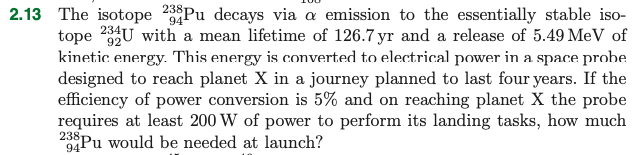
\includegraphics[scale = 0.5]{2.13.png}
\end{figure}

Looking at the required power and the power conversion efficiency, then we can find the total power $P_{\text{req}}$ we need to be released in the $\alpha$ emission:

\begin{align}
    P_{\text{req}} &= \frac{200\;\text{W}}{5\%}\\
    P_{\text{req}} &= 4000\;\text{W}
\end{align}

With the given released kinetic energy, we can then get the power $P_{\alpha}$ given by the $\alpha$ emission:

\begin{align}
    P_{\alpha} &= \mathcal{A}(t)\times 5.49 \text{MeV} \times \frac{1.602\times 10^{-13}\text{Ws}}{1\text{MeV}}
\end{align}

To find the power released in the $\alpha$ emission, we check its activity given by $\mathcal{A} (t) = \lambda N_0 \exp(-\lambda t)$. With the given mean lifetime $\tau$, then we can say that the decay constant $\lambda$ can be expressed as:

\begin{align}
    \lambda = \frac{1}{\tau}
\end{align}

thus using this, we get an expression for the activity:

\begin{align}
    \mathcal{A}(t) = \frac{1}{\tau} N_0 \exp(-t/\tau)
\end{align}

if we equate the power given by the reaction $P_{\alpha}$ and the power needed $P_{\text{req}}$, then we can arrive at a value for the initial number of $\; _{\;\;94}^{238}\text{Pu}\;\text{atoms}$ required ($N_0$):

\begin{align}
    4000\;\text{W} =\frac{1}{\tau} N_0 \exp(-t/\tau)\times 5.49 \text{MeV} \times \frac{1.602\times 10^{-13}\text{Ws}}{1\text{MeV}}
\end{align}

using the given $t=4\;\text{yrs}$ and $\tau =126.7\;\text{yrs}$ and converting them to seconds, we get:

\begin{align}
    4000\;\text{W} \times  
    \frac{1\text{MeV}}{1.602\times 10^{-13}\text{Ws}} \times 
    \frac{1}{5.49 \text{MeV}} \times \frac{126.7\;\text{yrs}}{\exp(-4/126.7)} \times \frac{365\;\text{days}}{1\;\text{yr}}\times \frac{24\;\text{hrs}}{1\;\text{day}} \times \frac{60\;\text{min}}{1\;\text{hr}}\times\frac{60\;\text{s}}{1\;\text{min}}  &=  N_0
\end{align}

\begin{align}
    N_0 = 1.88 \times 10^{25}\;\; _{\;\;94}^{238}\text{Pu}\;\text{atoms}
\end{align}

to get the needed weight $W$, then we use its molar mass: 

\begin{align}
    W = (1.88 \times 10^{25} \;\text{atoms})\times \frac{1\;\text{mol}}{6.02\times 10^{23}\;\text{atoms}} \times \frac{238\;\text{g}}{1\;\text{mol}} \times \frac{1\;\text{kg}}{1000\;\text{g}}
\end{align}

\begin{align}
\boxed{
    W = 7.43\;\text{kg}
}
\end{align}
\newpage
%==============================================================
\setcounter{equation}{0}
\begin{figure}[h!]
    \centering
    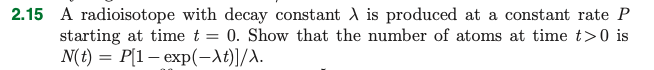
\includegraphics[scale = 0.55]{2.15.png}
\end{figure}

From the given decay constant $\lambda$ and rate $P$ starting at $t=0$, then we can express $dN(t)/dt$ as:

\begin{align}
    \frac{dN(t)}{dt} &= P - \lambda N(t)\\
    P &= \frac{dN(t)}{dt} + \lambda N(t)
\end{align}

to get the integrating factor $\mu$ to be multiplied to both sides for the differential equation $q(t) = y'+p(t)y$, we have:

\begin{align}
    \mu &= e^{\int p(t)\;dt}\\
    \mu &= e^{\int \lambda\; dt}\\
    \mu &= e^{\lambda t}
\end{align}
%the end result should have an exponential term, so there must be an exponential term inserted into the equation. We note that the derivative of $f(t)e^{\lambda t}$ with respect to $t$ is:

multiplying each side by $e^{\lambda t}$, we get:

\begin{align}
    Pe^{\lambda t} &= \frac{dN(t)}{dt}e^{\lambda t} + \lambda N(t)e^{\lambda t}\\
\end{align}

we note that the derivative of $f(t)e^{\lambda t}$ with respect to $t$ is:

\begin{align}
    \frac{d}{dt}[f(t)e^{\lambda t}] = f(t)\lambda e^{\lambda t} + e^{\lambda t} \frac{df(t)}{dt} 
\end{align}


noting that the right hand side looks similar to the derivative above, then we can rewrite it as:

\begin{align}
    Pe^{\lambda t} &= \frac{d N(t) e^{\lambda t}}{dt}
\end{align}

integrating both sides with respect to $t$, we get:

\begin{align}
    \int Pe^{\lambda t} dt &= \int \frac{d N(t) e^{\lambda t}}{dt}\\
    \frac{P}{\lambda} e^{\lambda t} + C &= N(t) e^{\lambda t}
\end{align}

to evaluate for the integration constant $C$, we note the condition $N(0)=0$. Thus at $t=0$ we get:

\begin{align}
    \frac{P}{\lambda} + C  &= 0\\
    C &= - \frac{P}{\lambda}
\end{align}

%\begin{align}
%    P\left( \frac{1}{\lambda} + C \right) &= 1\\
%    C &= \frac{1}{P} - \frac{1}{\lambda}
%\end{align}

using this integration constant, then our original equation becomes:

\begin{align}
    \frac{P}{\lambda} e^{\lambda t} - \frac{P}{\lambda}  &= N(t) e^{\lambda t}
\end{align}

\begin{align}
\boxed{
    N(t) = \frac{P \left(1 - e^{-\lambda t} \right)}{\lambda}
}
\end{align}

\end{document}